\section{Umsetzung}
Im Folgenden wird die Umsetzung insbesondere im
Bezug auf die Wahl der Technolgie sowie Darstellung
der App betrachtet.

\subsection{Technologie}
Um Apps zu entwickeln gibt es viele Möglichkeiten.
Diese lassen sich grob in folgende Arten einteilen

\begin{table}[htbp]
    \begin{tabular}{|l|l|}
    \hline
    Art      & Charakteristik                                                                                                                                                       \\ \hline
    Hybrid   & Web-Apps werden im nativen Kontext in einer WebView eingebunden                                                                                                      \\ \hline
    Native   & \begin{tabular}[c]{@{}l@{}}Adressieren konkrete Zielplattformen und deren Programmiersprachen.\\ Android (Java, Kotlin, Dart), iOS (Objective-C, Swift)\end{tabular} \\ \hline
    Web Apps & Über einen Server bereitgestellte plattformunabhängige Anwendungen                                                                                                   \\ \hline
    \end{tabular}
    \caption{Übersicht Arten von Apps}
\end{table}

Ich bin großer Fan von \ac{WORA} und entwickle überlicherweise vor allem Web-Apps.
Um etwas neues zu lernen und daran zu wachsen, entschied ich mich,
dieses Mal dazu eine Cross-Plattform-Technolgie zu nutzen.
Die Entscheidung fiel dabei auf das von Google entwickelte Open Source \ac{UI}-Kit \textit{Flutter}.

\begin{figure}[H]
    \minipage[t]{0.4\textwidth}
        
\includegraphics[width=\linewidth]{flutter_logo}
        \caption{ Flutter-Logo }
    \endminipage\hfill
    \minipage[t]{0.4\textwidth}
        
\includegraphics[width=\linewidth]{dart_logo}
        \caption{ Dart-Logo }
    \endminipage\hfill
\end{figure}

\subsection{Besonderheiten von Flutter}
\subsubsection{Performance}
Eine der Besonderheiten von \textit{Flutter} ist es, dass dieses UI-Kit weder eine WebView
noch die vom Betriebssystem mitgelieferten Widgets benutzt. Widgets sind in der
Welt von \textit{Flutter} alles von Bedienelemente bis hin zu Layout-Helfern.
Statt diese mitgelieferten Widgets zu nutzen, setzt \textit{Flutter} auf eine
eigene Rendering-Engine welche häufig mit einer 2D-Spiele-Engine verglichen wird.
Eines der Entwicklungsziele von \textit{Flutter} war es nämlich,
besonders performante Apps entwickeln zu können welche mit einer hohen
Hertz-Zahl (60-120 \textit{Hz}) laufen. Mit diesem Ansatz ist es möglich,
die gesamte UI über den Grafikchip des Systems zu berechnen und die CPU zu entlassen.

\subsubsection{Dart}
\textit{Flutter}-Apps werden in \textit{Dart} entwickelt.

\subsubsection{Deklaratives UI}
Im Gegensatz zu imperativen Frameworks wie dem \textit{Android SDK}
oder dem \textit{iOS UiKit} handelt es sich bei \textit{Flutter} um
ein so genanntes deklaratives Framework. Dies bedeutet,
dass das UI von Flutter immer akutellen \textit{"State"} reflektiert.
Wird beispielsweise eine Option in den Einstellungen einer App geändert,
so ändert sich der \textit{"State"} der App welches das Neuzeichnen
der App auslöst (eine Checkbox wird gefüllt, ein Switch aktiviert).
Imperativ würde bedeuten, dass es Methoden wie \textit{widget.setText}
gibt um Werte direkt zu ändern. Hier wird der \textit{"State"} geändert
und das UI wird komplett neu gezeichnet.

\paragraph{Technisches Beispiel}\mbox{}
\hfill
\break

\begin{figure}[H]
    \centering
    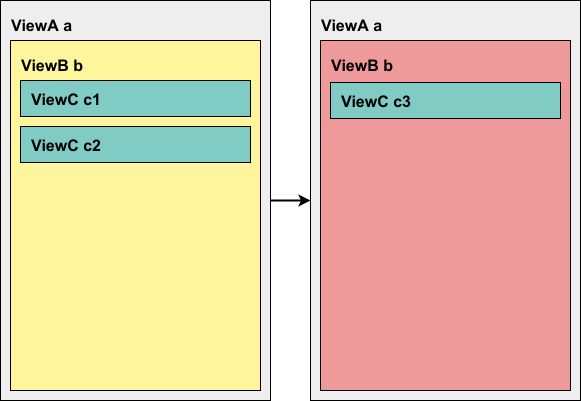
\includegraphics[width=0.8\columnwidth]{declarative_ui_example}
    \caption{Vergleich deklaratives \& imperatives UI}
\end{figure}

Im imperativen Stil würde man eine Instanz \textit{b} des so
genannten \textit{Owners} der View \textit{ViewB} nutzen
und mit Hilfe eine Selektors wie beispielsweise \textit{findViewById}
Änderungen auf dieser anwenden (und somit diese implizit invalidieren).
Das kann ungefähr so aussehen:

\begin{figure}[H]
    \centering
    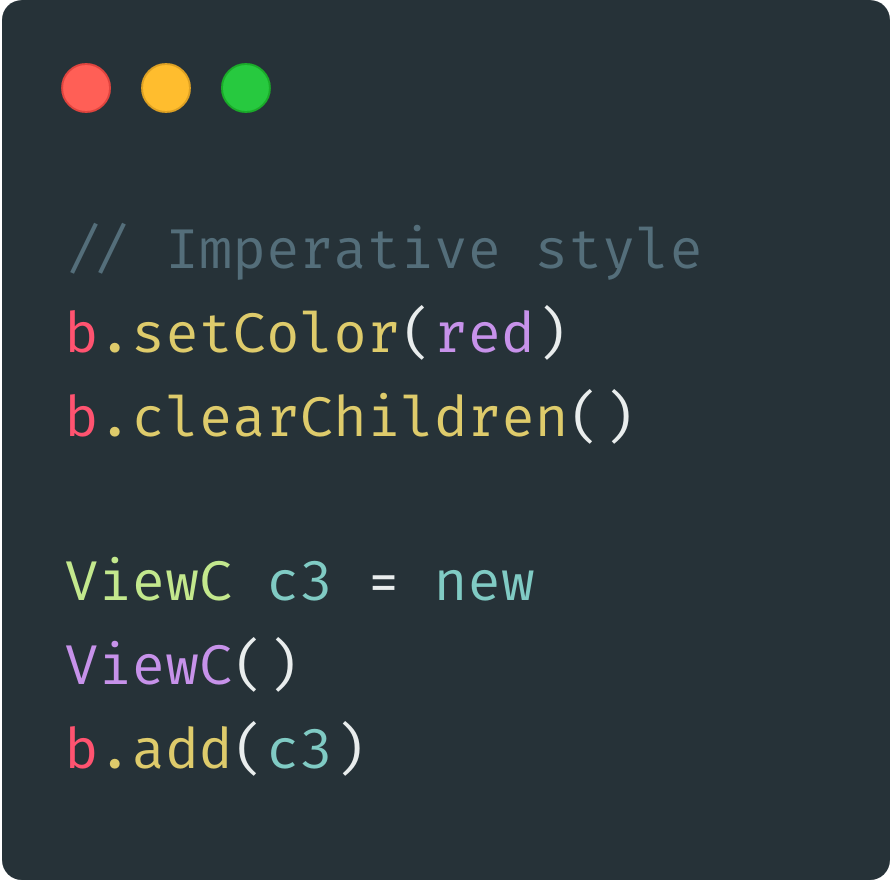
\includegraphics[width=0.4\columnwidth]{imperative_style}
    \caption{Beispiel: imperativer Stil}
\end{figure}

Außerdem müsste dieses Setup im Konstruktor von \textit{ViewB} dupliziert
werden, da die UI (der \ac{SPOT}) möglicherweise die Instanz \textit{b} überlebt.
Im deklarativen Frameworks sind View-Konfigurationen
(wie \textit{Flutter's} Widgets) unveränderlich (immutable) und an sich
nur simple Blaupausen. Um ein UI zu ändern, löst ein Widget einen Rebuild
auf sich selbst aus (in \textit{StatefulWidgets} häufig per \textit{setState()}
und erzeugt damit einen neuen Widget-Subtree.

\begin{figure}[H]
    \centering
    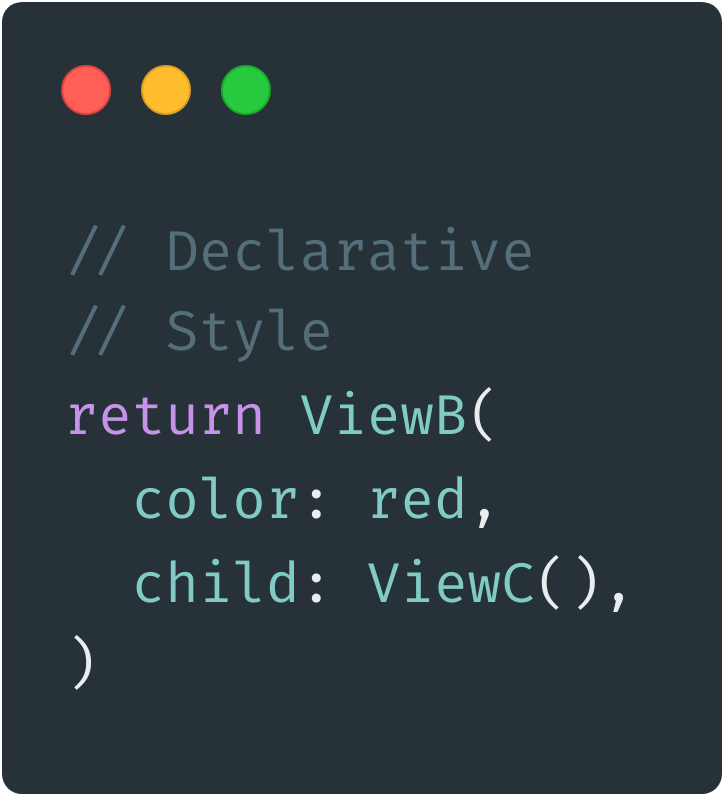
\includegraphics[width=0.4\columnwidth]{declarative_style}
    \caption{Beispiel: deklarativer Stil}
\end{figure}



\subsection{Herausforderungen}
\subsubsection{Date-Library}

\subsection{Widgets}
\subsubsection{PizzaItem}
